\section{Metoda przeprowadzenia badań}
Badanie zostało przeprowadzone jako badanie internetowe. Trwało dokładnie jeden miesiąc od 29 IV do 29 V 2011. Do przygotowania ankiety zostały użyte polskie tłumaczenia \emph{Job Satisfaction Survey} oraz \emph{Utrecht Work Engagement Survey} przygotowane przez \href{http://www.psychologia.amu.edu.pl/ip-uam/struktura-zatrudnienia-w-instytucie/curriculum-vitae-teresa-chirkowska-smolak/}{dr Teresę Chirkowską-Smolak} (w załączniku pełna treść pytań \ref{sec:jss-text} oraz \ref{sec:uwes-text}). Pytania zostały wprowadzone do instancji darmowego oprogramowania do przeprowadzania ankiet
w Internecie -- \href{http://www.limesurvey.org/}{LimeSurvey}. Ankieta jest nadal dostępna pod
adresem \url{survey.alewandowska.pl}.

\begin{figure}[h]
\begin{center}
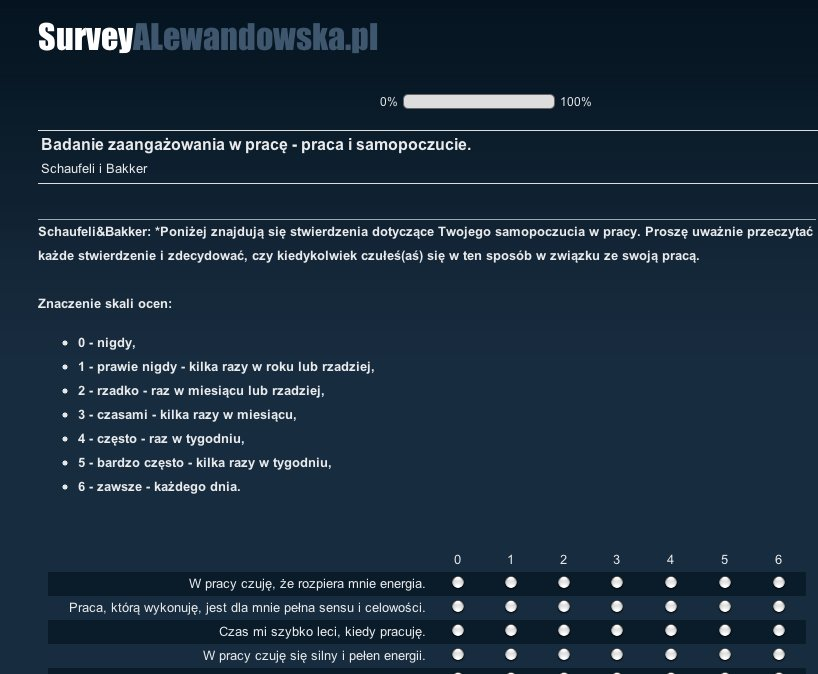
\includegraphics[width=0.8\textwidth]{survey}
\end{center}
\caption{Wygląd pierwszej strony ankiety internetowej z pytaniami.}
\label{fig:sex}
\end{figure}

Odnośnik do gotowej ankiety internetowej został rozesłany drogą emaliową na listy emaliowe kilku instytucji i organizacji, w tym:
\begin{itemize}
\item na listę absolwentów kierunku Informatyka na Wydziale Informatyki i Zarządzania Politechniki Poznańskiej -- rok ukończenia 2008,
\item na listę pracowników Poznańskiego Centrum Superkomputerowo-Sieciowego,
\item na listę pracowników Allegro.
\end{itemize}
Oczywiście wszyscy byli zachęcani do rozsyłania ankiety dalej, więc osoby biorące udział w badaniu nie muszą, ale mogą być ograniczone tylko do wskazanych firm. Wypełnienie ankiety było dobrowolne, przy czym wszystkie pytania w ankiecie były obowiązkowe, także dotyczące danych demograficznych.
